\section{Approach}
In this section, we first revisit CLIP and denote some basic concepts, such as image-text contrastive supervision (i.e., the InfoNCE loss). 
Next, we present the overview of our \workname framework. 
Then we introduce every auxiliary supervision: Self-Supervision(SS), Multi-View Supervision(MVS), and Nearest-Neighbor Supervision(NNS).


\begin{figure}[t]
	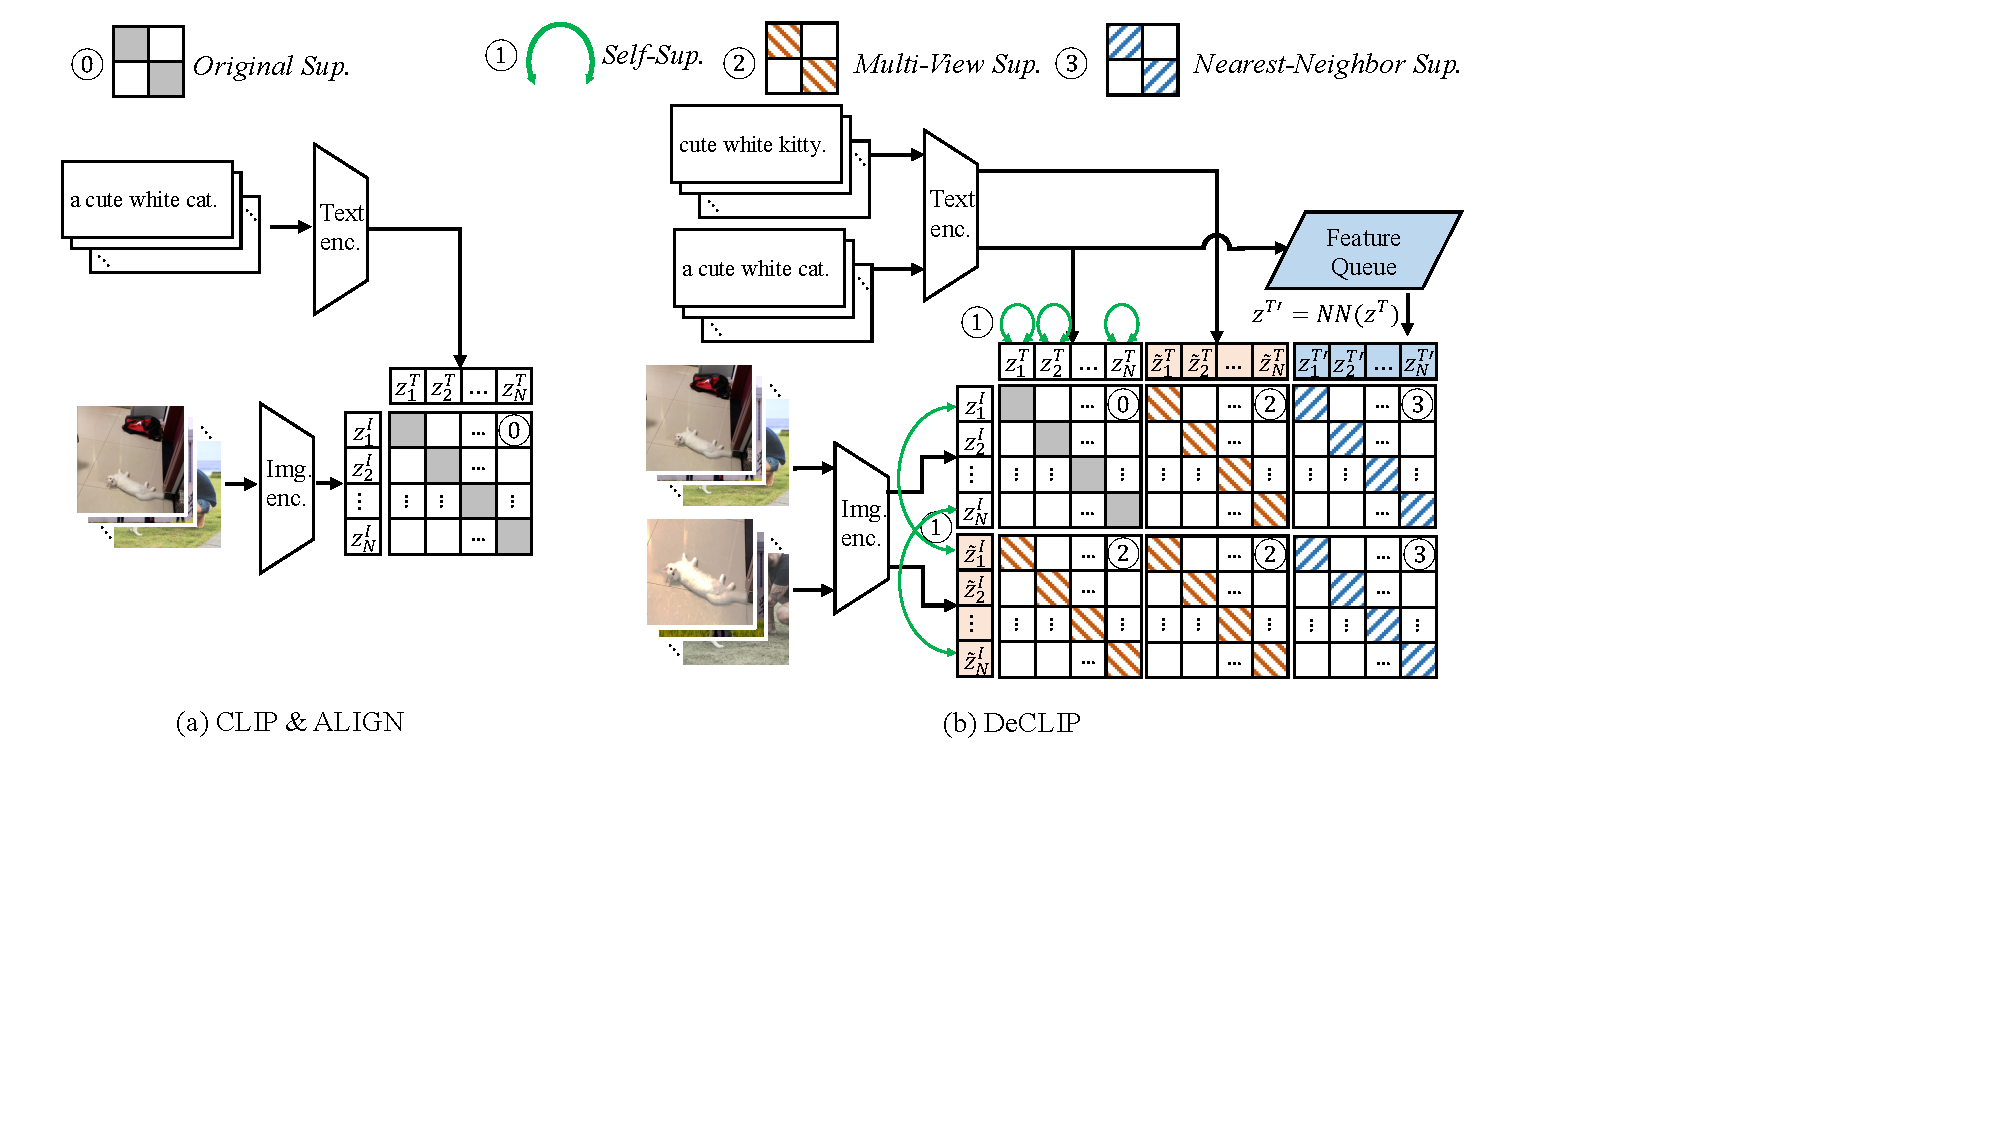
\includegraphics[width=0.99\columnwidth]{DeCLIP/figs/main_figure.pdf}
    % \vskip -0.15in
	\caption{
	%Our \workname has two augmented views for both image and text.
% 	We first extract structural information within each modality using Self-Supervision (SS \protect\circled{1}). 
	%We first adopt the instance discrimination contrastive learning and Masked Language Modeling (MLM) to extract structural information within image and language modality, respectively (SS \protect\circled{1}).
% 	Worth mentioning, language SS is utilized via Masked Language Modeling (MLM), which is omitted in this figure. 
	%Cross-modal Multi-View Supervision (MVS \protect\circled{2}) helps to learn more robust features. We also learn from other pairs via Nearest-Neighbor Supervision (NNS \protect\circled{3}). \wl{(This caption does not help me to understand the overall method.)}
	(a) CLIP and ALIGN jointly train an image encoder and a text encoder to predict the correct pairings of a batch of (image, text) training examples.
% 	indicates the original image-text contrastive supervision for the CLIP and ALIGN. 
    (b) Our \workname overview. 
% 	In \workname, we additionally add three types of supervision.
% 	\protect\circled{1} means Self-Supervision(SS) within each modality, in which image self-supervision is SimSiam and text self-supervision is MLM.
    \protect\circled{1} means \textcolor[RGB]{0,153,51}{Self-Supervision(SS)}. For image SS, we maximize the similarity between two augmented views of the same instance. For text SS, we leverage Masked Language Modeling(MLM) within a text sentence.
    % , in which we additionally use the siamese representation learning from SimSiam~\citep{chen2021exploring} for image self-supervision and Masked Language Modeling(MLM) from Bert~\citep{devlin2018bert} for text self-supervision.
	\protect\circled{2} represents cross-modal \textcolor[RGB]{204,102,51}{Multi-View Supervision(MVS)}. We first have two augmented views of both image and text, then contrast the $2\times2$ image-text pairs.
% 	in which we introduce the $2\times2$ image-text pairs for additional supervision after extracting two views of both image and text from stochastic data augmentations.
	\protect\circled{3} indicates \textcolor[RGB]{0,102,153}{Nearest-Neighbor Supervision(NNS)}. We sample text NN in the embedding space to serve as additional supervision. 
% 	in which we propose the additional text supervision from other high-quality text descriptions by using the nearest neighbor of the text descriptions from a queue for each image-text pair.
	The combination of the three supervision leads to efficient multi-modal learning. }
	\label{fig:main_figure}
\end{figure}

\subsection{Revisiting CLIP}

Contrastive Language-Image Pre-training (CLIP)~\citep{radford2021learning} aims to learn directly from the raw text about images. They use a dual-encoder architecture as in Fig.~\ref{fig:main_figure}(a). 
% CLIP~\citep{radford2021learning} uses a dual-encoder architecture as in Fig.~\ref{fig:main_figure}(a). 
The model consists of an image encoder (e.g., CNN~\citep{he2016deep} or ViT~\citep{dosovitskiy2020image}) and a text encoder(e.g., Transformer~\citep{vaswani2017attention} or its variants~\citep{radford2019language}), with a multimodal interaction at the top. 
The image and text features are projected to the same dimension and followed by L2 normalization before interaction.
At the training phase, a contrastive objective pushes the embeddings of matched image-text pairs together while pushing those of non-matched pairs apart. 
In a batch of $N$ image-text pairs ${\{(\bm x_i^I, \bm x_i^T)\}}$, we denote $\bm x_i^I$ and $\bm x_i^T$ as image and text of the $i_{th}$ pair. Let $\bm z_i^I$ and $\bm z_j^T$ be the normalized embedding of the $i_{th}$ image and $j_{th}$ text, respectively. CLIP uses InfoNCE loss~\citep{oord2018representation}. The loss for the image encoder can be denoted as Eq.~\ref{eq:infonce}.

\begin{equation}
\label{eq:infonce}
    L_I = - \frac{1}{N} \sum_{i=1}^{N} \log \frac{\exp(\mathrm{sim}(\bm z_i^I, \bm z_i^T)/\tau)}{\sum_{j=1}^{N}\exp(\mathrm{sim}(\bm z_i^I, \bm z_j^T)/\tau)}~
\end{equation}

Here, the similarity function $\mathrm{sim}(,)$ is measured by dot product, and $\tau$ is a learnable temperature variable to scale the logits. We have a symmetrical loss for image and text encoder, thus the overall loss function $L_{CLIP}$ is the average of $L_I$ and $L_T$.

% \begin{equation}
% \label{eq:cliploss}
%     L = \frac{1}{2} (L_I + L_T)~
% \end{equation}

At the test phase, the learned text encoder synthesizes a zero-shot linear classifier by embedding the arbitrary categories of the test dataset. Because it is rare in the dataset that image caption is just a single word, CLIP uses prompts to make up the context of the category \texttt{\{label\}}, such as \texttt{"a photo of a \{label\}"}. Unless otherwise specified, we use the same prompt engineering and ensembling techniques as CLIP. Details can be found in Appendix~\ref{Prompts}.

\subsection{Overview of \workname}

As shown in Fig.~\ref{fig:main_figure}(b), our \workname has three additional supervisory signals. 

% \checkme{3.2 description fig3}
\protect\circled{1}  We first use existing methods to exploit image and text Self-Supervision (SS) within its modality. 
For image SS, we adopt the simple yet effective SimSiam~\citep{chen2021exploring}.
% Here, we denote $(z^I, \tilde{z}^I)$ as image features of two augmented views. 
The objective is to maximize the similarity between two augmented image features.
% More specifically, we maximize the similarity between two augmented views of the same instance, e.g. ($(z_1^I, z_1^I)$)
% the instance discrimination contrastive learning framework to learn a more common-sense representation. 
% More specifically, we use the simple yet effective SimSiam~\citep{chen2021exploring} in this paper. 
For text SS, we adopt the most widely used Masked Language Modeling (MLM)~\citep{devlin2018bert} as the pre-text task. 
We believe other kinds of self-supervised learning algorithms (e.g. MoCo~\citep{he2020momentum}, SimCSE~\citep{gao2021simcse} are orthogonal with our framework.

\protect\circled{2} While SS only focuses on a single modality, we further propose cross-modal Multi-View Supervision (MVS).
We apply stochastic data augmentations for both images and texts, resulting in two correlated views\footnotemark[1] of each example.
Then, the image-text contrastive loss is calculated for all the $2\times2$ pairs.
Worth mentioning, the original CLIP does not use text augmentations and only uses random square crop image augmentations, thereby is data-hungry.
The extension is instinctive and straightforward. Specifically, we contrast the $2\times2$ pairs and resulting in $3\times$ more additional supervision.


% \begin{wrapfigure}{o}{0.37\textwidth}
% \vspace{-2.5em}
%     \begin{center}
%     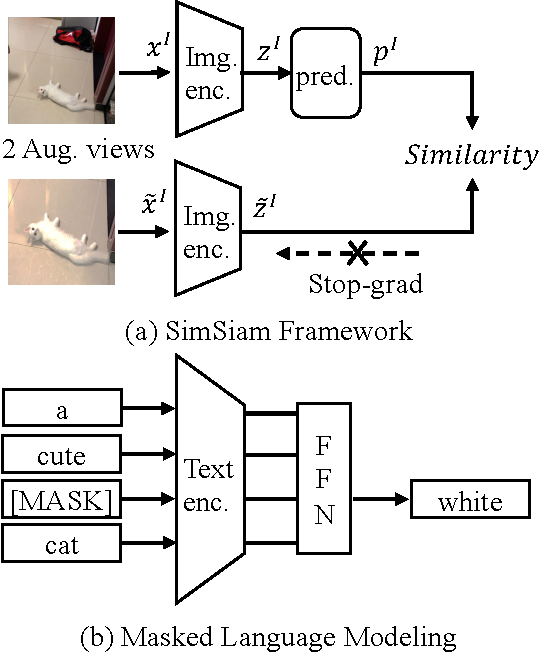
\includegraphics[width=\linewidth]{DeCLIP/figs/self-supervision.pdf}
%     \end{center}
%     \vspace{-1em}
%         \caption{Self-Supervision with each modality. We adopt SimSiam and MLM for image and text SS.}
%         \vspace{-2em}
%     \label{fig:self-supervision}
%         \vspace{-2em}
% \end{wrapfigure}


\protect\circled{3} We also propose novel Nearest-Neighbor Supervision (NNS) mined in embedding space to make better use of similar text descriptions among the dataset.
In detail, we maintain a first-in-first-out feature queue that is representative of the whole data distribution. We use the nearest-neighbor search in embedding space to get the semantically similar text descriptions. Then we use the image-text contrastive loss to get additional supervision. 

% \wl{(Use this to illustrate what it is, not why it is so).} To mitigate the noise in the image-text pairs, we leverage nearest neighbors (NN) mined in embedding space. 
% The NN supervision is mainly based on the intuition that one image is likely to have other high-quality text descriptions among the dataset besides its paired text.
% It is infeasible to search neighbors within the entire million-scale dataset. 
% Therefore, we maintain a first-in-first-out feature queue that is representative of the whole data distribution.

% \begin{enumerate}[label=\protect\circled{\arabic*}, leftmargin=*]
%     \item We first use existing methods to exploit image and language self-supervision within its own modality. 
%     For image, we adopt the instance discrimination contrastive learning framework to learn a more common-sense representation. 
%     More specifically, we use the simple yet effective SimSiam~\citep{chen2021exploring} in this paper. 
%     For language, we adopt the most widely used Masked Language Modeling (MLM)~\citep{devlin2018bert} pre-text task. 
%     We believe other kinds of self-supervised learning algorithms (e.g. MoCo~\citep{he2020momentum}, SimCSE~\citep{gao2021simcse} are orthogonal with our framework.
    
%     \item While SS is focusing on a single modality, we further propose the Multi-View Supervision (MVS) in the multi-modal setting. 
%     We apply stochastic data augmentations for both images and texts, resulting in two correlated views\footnotemark[1] of each example.
%     Worth mentioning, original CLIP does not use text augmentations and only uses random square crop image augmentations, thereby is data-hungry. 
%     The extension is instinctive and straightforward. 
%     Specifically, we contrast the $2\times2$ pairs resulting $3\times$ more additional supervision. \wl{(after reading this, I cannot understand what is MVS).}
%     \item \wl{(Use this to illustrate what it is, not why it is so).} To mitigate the noise in the image-text pairs, we leverage nearest neighbors (NN) mined in embedding space. 
%     The NN supervision is mainly based on the intuition that one image is likely to have other high-quality text descriptions among the dataset besides its paired text.
%     It is infeasible to search neighbors within the entire million-scale dataset. 
%     Therefore, we maintain a first-in-first-out feature queue that is representative of the whole data distribution.
% \end{enumerate}


% \textbf{TODO: Add loss in description} In summary, our overall objective can be denoted as Eq.~\ref{eq:overall_loss}. 

% \begin{equation}
% \label{eq:overall_loss}
%     L_{\workname} = (1 - \alpha - \beta - \gamma)L_{CLIP} + \alpha L_{SS} + \beta L_{MVS} + \gamma L_{NS}
% \end{equation}


\subsection{Supervision exists everywhere}

% \subsubsection{Self-supervision within each modality}
\paragraph{Self-Supervision within each modality}
% \paragraph{Image SS.} 
\begin{wrapfigure}{o}{0.37\textwidth}
\vspace{-2.5em}
    \begin{center}
    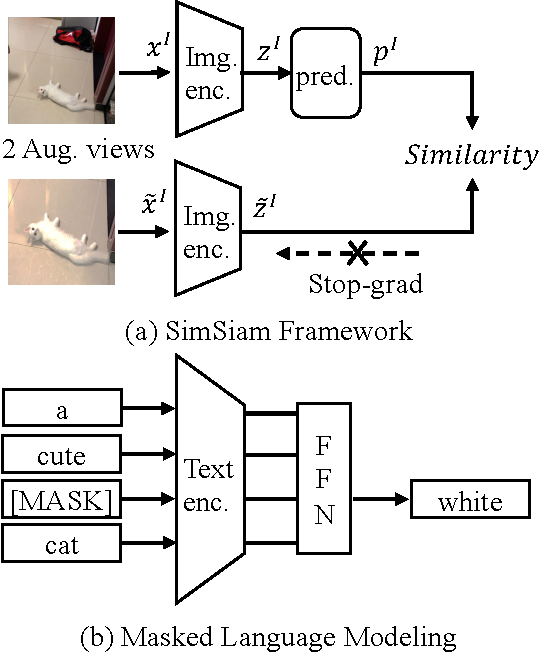
\includegraphics[width=\linewidth]{DeCLIP/figs/self-supervision.pdf}
    \end{center}
    \vspace{-1em}
        \caption{Self-Supervision with each modality. We adopt SimSiam and MLM for image and text SS.}
        \vspace{-2em}
    \label{fig:self-supervision}
        % \vspace{-2em}
\end{wrapfigure}

Following SimSiam~\citep{chen2021exploring} (depicted in Fig~\ref{fig:self-supervision}(a)), we first have two augmented views ($x^I$, $\tilde{x}^I$) for each image. 
These two views are sent to the image encoder (weights are shared between views). 
We also use the popularized nonlinear predictor module, which is typically a 2-layer MLP, to improve the representation quality in the encoder~\citep{chen2020simple}. 
The objective is to maximize the similarity between $\tilde{z}^I$ and $p^I$, which is a negative cosine similarity in this paper. To avoid the trivial “collapsing” solution, we follow ~\citep{chen2021exploring} to adopt a stop-grad technique. 

% However, other related methods (e.g. MoCo~\citep{he2020momentum, chen2020improved}) are applicable in our \workname as well. 
% The augmented two views are sent to an encoder network $f$ of each modality. It is worth to mention that the encoder network shares weights between two views. We use the popularized nonlinear predictor module $h$, typically a 2-layer MLP, \checkme{to maintain more information in encoder~\citep{chen2020simple}.} 
% The objective is to maximize the similarity between $\widetilde{z}$ and $h(z)$. \checkme{some functions here.} An undesired trivial solution to Siamese networks is all outputs “collapsing” to a constant. To mitigate this problem, we follow ~\citep{chen2021exploring} to adopt a stop-grad technique. For more details, \checkme{Details can be found in the Appendix.} please check our pseudo code at Appendix \ref{Pseudo Code}

% \paragraph{Language SS.} 
% Here we follow the original BERT~\citep{devlin2018bert}.... Some details here.
% More details can be found in ~\checkme{Appendix XXX}. Here we follow the original BERT~\citep{devlin2018bert}.... Some details here.
% More details can be found in ~\checkme{Appendix XXX}. Here we follow the original BERT~\citep{devlin2018bert}.... Some details here.
As shown in Fig.~\ref{fig:self-supervision}(b), we follow the method in BERT~\citep{devlin2018bert} for our text self-supervision. In detail, we first randomly choose $15\%$ of all tokens in each sequence. Then the token is replaced with (1) the \texttt{[mask]} token $80\%$ of the time (2) a random token $10\%$ of the time (3) the unchanged token $10\%$ of the time. Then, the output of the language module for the corresponding token is used to predict the original token with cross-entropy loss.
% More details can be found in ~\checkme{Appendix XXX}.

% \begin{figure}[t]
%     \begin{minipage}[t]{0.39\linewidth}
% 	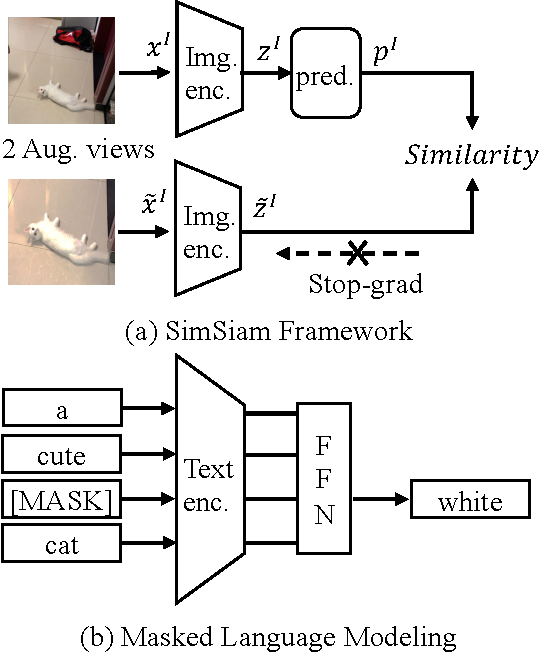
\includegraphics[width=0.99\columnwidth]{DeCLIP/figs/self-supervision.pdf}
% 	\caption{Self-Supervision with each modality. We adopt SimSiam and MLM for image and language SS.}
% 	\label{fig:self-supervision}
% 	\end{minipage}%
%     \begin{minipage}[t]{0.59\linewidth}
% 	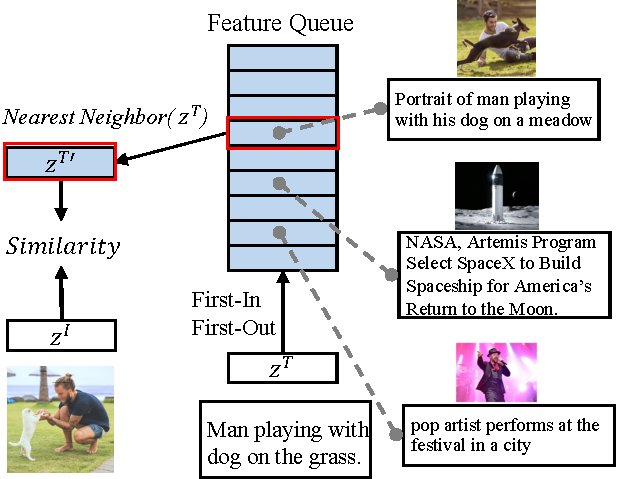
\includegraphics[width=0.99\columnwidth]{DeCLIP/figs/nearest_neighbor_supervision.pdf}
% 	\caption{Nearest-Neighbor Supervision. $z^{T'}$ is the NN of feature $z^T$ in the embedding space (FIFO feature queue). $z^{T'}$ will serve as an additional objective for $z^I$.}
% 	\label{fig:neighbor-supervision}
% 	\end{minipage}%
% \end{figure}


% \subsubsection{Multi-View Supervision}
\paragraph{Multi-View Supervision}
\label{sec:mvs}
The authors only contrast the original text (w/o augmentation) with a single `global view' of the image in the original CLIP. 
However, the text annotation of the image might not describe the whole picture, instead depicts a small local view of this image. 
For instance, as shown in the image with the text \texttt{"a cute white cat"} in Fig.~\ref{fig:main_figure}, the central concept (cat) only occupies a small part of the picture.
To mitigate this discrepancy, we get a closer look at the local region and utilize it as our auxiliary supervision, as shown in the augmented view in Fig.~\ref{fig:main_figure}(b). This intuitive idea is akin to the successful \texttt{Multi-crop} transformation~\citep{caron2020unsupervised, van2021revisiting} in image SSL. 
We further extend it into the multi-modal setting. 
More specifically, we reuse the two image views introduced in SS, which contains the \texttt{RandomResizedCrop} policy to obtain a small local view.
For text, as our goal is to understand the overall semantic meaning of a sentence, we adopt text classification augmentation EDA~\citep{wei2019eda} to generate two text views. 
Besides the original contrastive loss between (${z}^I, {z}^T$), we can contrast (${z}^I, \tilde{z}^T$), ($\tilde{z}^I, {z}^T$) and ($\tilde{z}^I, \tilde{z}^T$), leading to $3\times$ diverse and high-quality additional supervision.
% Because of these $2\times2$ augmented views, we can contrast ()
% We contrast the original image feature($\tilde{z}^I$) with two augmented text views and vice versa.
% These $2\times2$ augmented views can provide $3\times$ diverse and high-quality additional supervision, thus leading to more robust representations. 
More conveniently, they are naturally compatible with the image-text contrastive loss as denoted in Eq.~\ref{eq:infonce}.

% \subsubsection{Nearest-Neighbor Supervision}
\paragraph{Nearest-Neighbor Supervision}
\begin{wrapfigure}{o}{0.42\textwidth}
\vspace{-1.8em}
    \begin{center}
    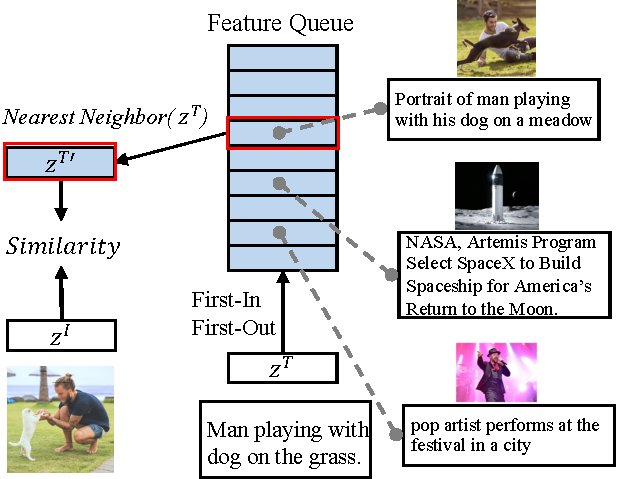
\includegraphics[width=\linewidth]{DeCLIP/figs/nearest_neighbor_supervision.pdf}
    \end{center}
    \vspace{-1.em}
        \caption{Nearest-Neighbor Supervision. $z^{T'}$ is the NN of feature $z^T$ in the embedding space. $z^{T'}$ will serve as an additional objective for $z^I$. We use the feature-level nearest neighbor for the text descriptions as the supervision.}
        % \vspace{-3em}
    \label{fig:neighbor-supervision}
        \vspace{-1em}
\end{wrapfigure}

As shown in Fig~\ref{fig:NN-supervision-small}, one image is likely to have other similar text descriptions among the dataset. 
% For example, in Fig.~\ref{fig:neighbor-supervision}, there is an image paired with the text \texttt{"Man playing with dog on the grass"}. 
% Another text \texttt{"Portrait of man playing with his dog on a meadow"} is also a perfect fit for this image.
To harness the information from other pairs and go beyond single pairs, we propose using nearest-neighbor (NN) to obtain more diverse supervision. 
More formally, we aim to find the NN feature $z^{T'}$ of text feature $z^T$ in the embedding space.
The distance between two features could be measured by a simple cosine similarity.
It is infeasible to search NN in the whole million-scale dataset. 
Thus, we maintain a FIFO queue $Q$ to simulate the whole data distribution. 
The size of $Q$ is 64K in our implementation.
As shown in Fig.~\ref{fig:neighbor-supervision}, we further get the contrastive loss between (${z}^I, z^{T'}$).
% contrast the image feature $z^I$ with $z^T$'s NN $z^{T'}$. 
Since there are two augmented image features, we also calculate the contrastive loss between ($\tilde{z}^I, z^{T'}$).
Fortunately, NNS is also compatible with Eq.~\ref{eq:infonce}.


In summary, we denote $L_{ISS}$ and $L_{TSS}$ as the loss function of image SS and text SS, respectively. $L_{MVS}$ is multi-view loss, and $L_{NNS}$ is nearest-neighbor loss. We have the overall loss function of our \workname as in Eq.~\ref{eq:overall_loss}.

\begin{equation}
\label{eq:overall_loss}
    L_{\workname} = (1 - \alpha - \beta - \gamma) L_{CLIP} + \alpha (L_{ISS} + L_{TSS}) + \beta L_{MVS} + \gamma L_{NNS}
\end{equation}